\documentclass{standalone}
\usepackage{tikz}
\usepackage{ctex,siunitx}
\setCJKmainfont{Noto Serif CJK SC}
\usepackage{tkz-euclide}
\usepackage{amsmath}
\usetikzlibrary{patterns, calc}
\usetikzlibrary {decorations.pathmorphing, decorations.pathreplacing, decorations.shapes,}

\begin{document}
\small
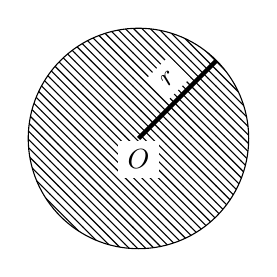
\begin{tikzpicture}[>=stealth,scale=0.7]
  \tkzSetUpPoint[fill=black]
  % \useasboundingbox(-1,-0.75)rectangle(3.7,1.4);
  \draw[pattern=north west lines] (0,0) circle (2);
  \draw[ultra thick] (0,0)node[below, fill=white]{$O$}--(45:2);	
  \node at (60:1.5) [left, rotate=45, fill=white]{$r$};
\end{tikzpicture}
\end{document}